\section{Modello Analitico}
%%%%%%%%%%%%%%%%%%%%%%%%%%%%%%%%%%%%%%%%%%%%%%%%%%%%%%%%%%%%%%%%%%%%%%%%%%%%%%%%
%%%%%%%%%%%%%%%%%%%%%%%%%%%%%%%%%%%%%%%%%%%%%%%%%%%%%%%%%%%%%%%%%%%%%%%%%%%%%%%%
\begin{frame}
\frametitle{Modello Analitico: Catena di Markov}

\begin{figure}[!h]
\centering
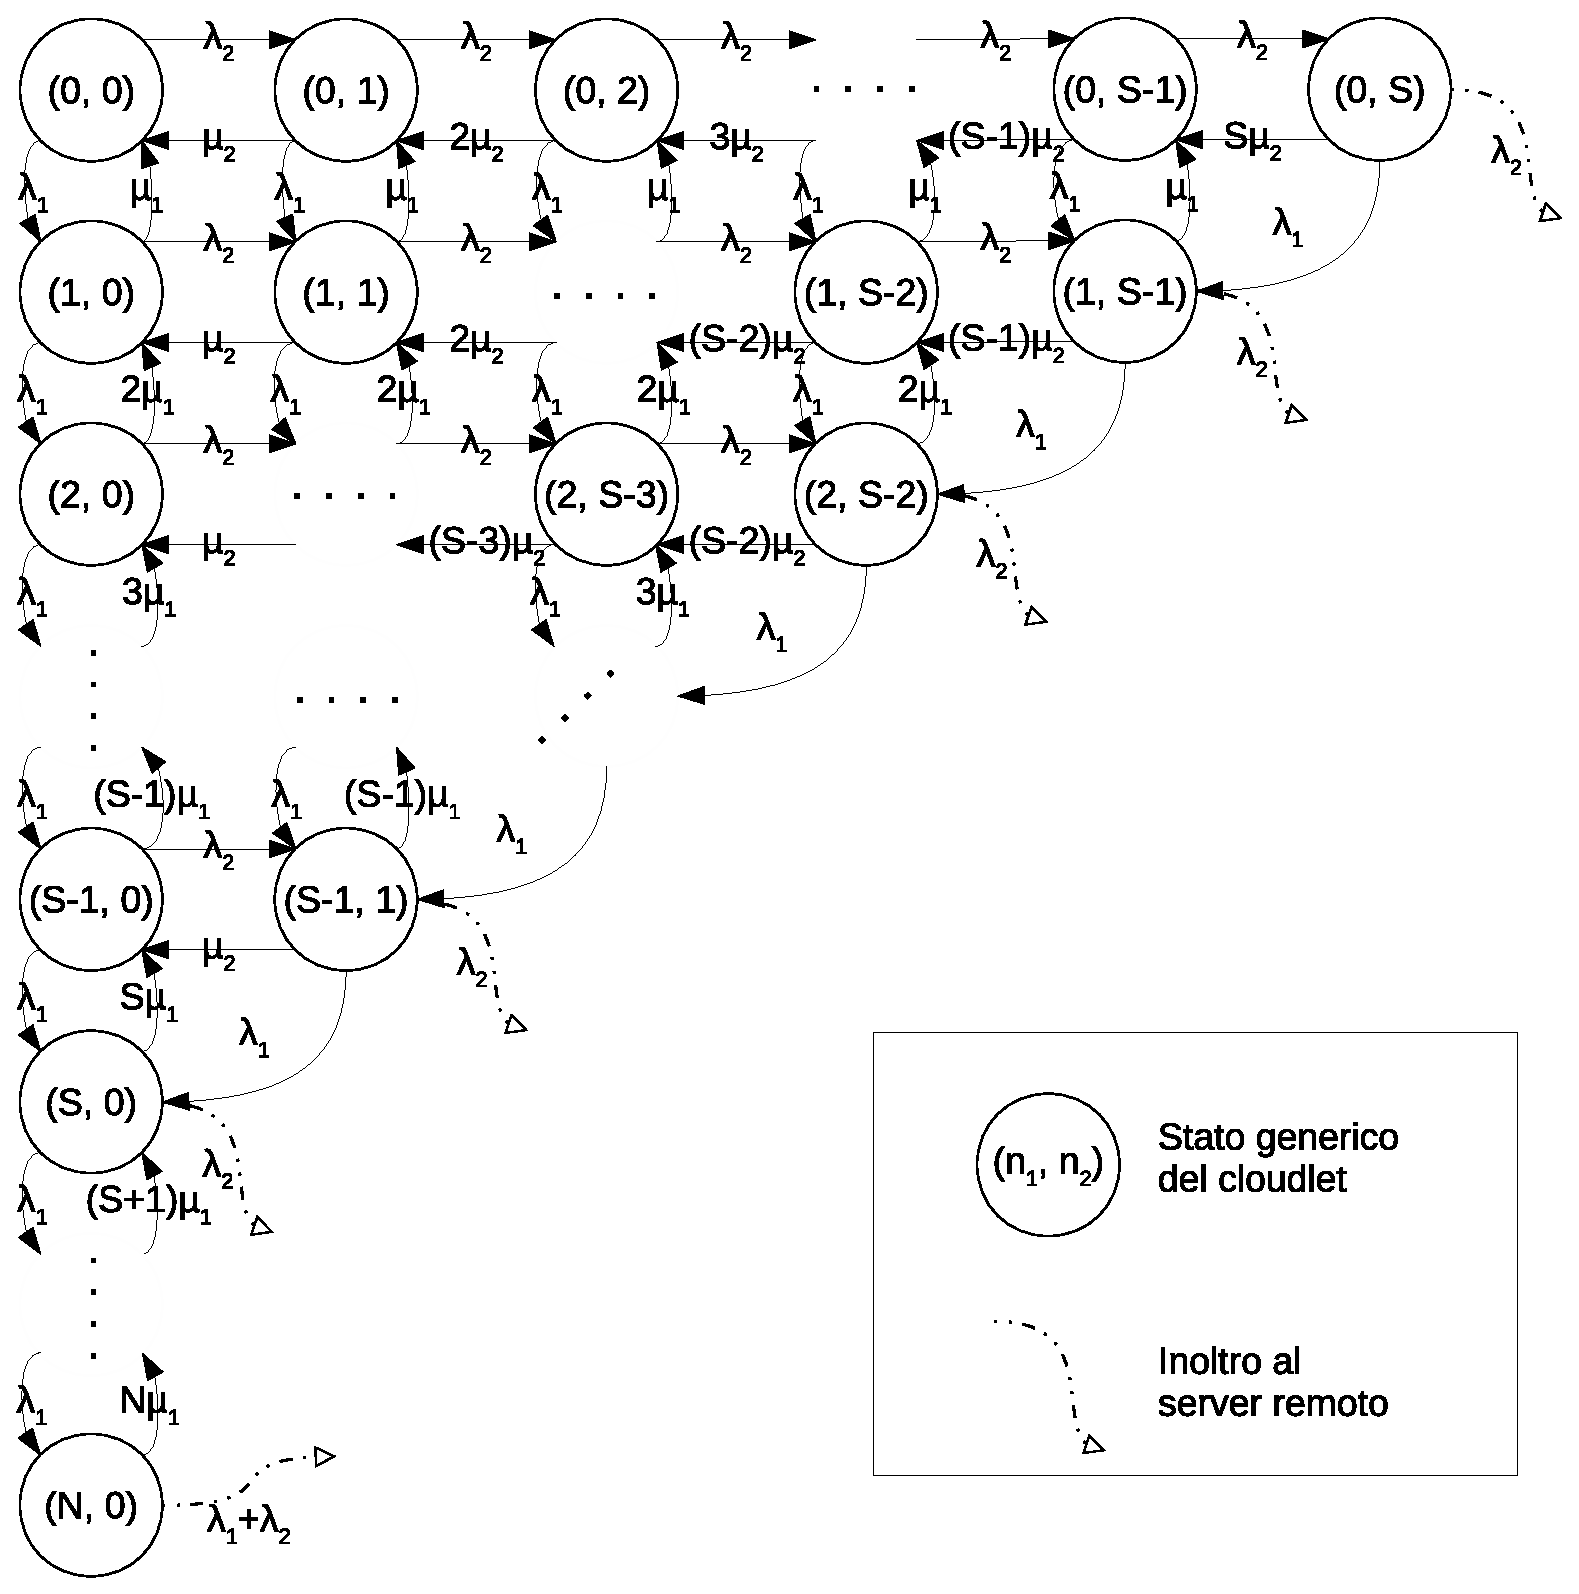
\includegraphics[width=0.7\textwidth]{../figures/ctmc}
\label{ctmc}
\end{figure}

\end{frame}
%%%%%%%%%%%%%%%%%%%%%%%%%%%%%%%%%%%%%%%%%%%%%%%%%%%%%%%%%%%%%%%%%%%%%%%%%%%%%%%%
%%%%%%%%%%%%%%%%%%%%%%%%%%%%%%%%%%%%%%%%%%%%%%%%%%%%%%%%%%%%%%%%%%%%%%%%%%%%%%%%
\begin{frame}
\frametitle{Modello Analitico: Probabilità Preliminari}
\begin{columns}
\column{.5\textwidth}
\begin{itemize}
\item \emph{Probabilità di Accettazione}
\begin{displaymath}
\Pi_A = \sum_{\substack{n_1,n_2:\\n_1 + n_2 < S}} \pi_{(n_1,n_2)}
\end{displaymath}
\item \emph{Probabilità di Soglia}
\begin{displaymath}
\Pi_S = \sum_{\substack{n_1,n_2:\\ n_1 + n_2 \geq S}} \pi_{(n_1,n_2)}
\end{displaymath}
\item \emph{Probabilità di Blocco}
\begin{displaymath}
\Pi_B = \sum_{\substack{n_1,n_2:\\n_1 + n_2 = N}} \pi_{(n_1,n_2)}
\end{displaymath}
\end{itemize}

\column{.5\textwidth}
\begin{itemize}
\item \emph{Probabilità di Interruzione}
\begin{displaymath}
\Pi_I = \sum_{\substack{n_1,n_2:\\n_1 + n_2 = N\\n_2 > 0}} \pi_{(n_1,n_2)}
\end{displaymath}
\item \emph{Probabilità di Interruzione a seguito di Accettazione}
\begin{displaymath}
P_{intr}^{clet} = \frac{\lambda_1 \ \Pi_I}{\lambda_2 \ \Pi_A}
\end{displaymath}
\item \emph{Probabilità di Interruzione di un job di classe 2}
\begin{displaymath} P_{intr} = \Pi_A \ P_{intr}^{clet}
\end{displaymath}
\end{itemize}
\end{columns}
\end{frame}
%%%%%%%%%%%%%%%%%%%%%%%%%%%%%%%%%%%%%%%%%%%%%%%%%%%%%%%%%%%%%%%%%%%%%%%%%%%%%%%%
%%%%%%%%%%%%%%%%%%%%%%%%%%%%%%%%%%%%%%%%%%%%%%%%%%%%%%%%%%%%%%%%%%%%%%%%%%%%%%%%
\begin{frame}
\frametitle{Modello Analitico: Throughput}
\begin{displaymath}
\lambda_1^{cloud} = \Pi_B \ \lambda_1 
\qquad\quad\qquad
\lambda_2^{cloud} = \lambda_{setup} = (\Pi_S + P_{intr}) \ \lambda_2 
\end{displaymath}
%
\setlength\arraycolsep{2pt}
\begin{eqnarray*}
X_j^{cloud} &=& \lambda_j^{cloud}   \qquad\quad\qquad\quad j=1,2 \\
X_{cloud} &=& \lambda_1^{cloud} + \lambda_2^{cloud}   \\
X^{setup} &=& \lambda_{setup}   \\
X_j &=& \lambda_j  \ \quad\qquad\quad\qquad \ \quad j=1,2 \\
X &=& \lambda \\
X_j^{clet} &=& X_j - X_j^{cloud} \ \qquad\quad j=1,2 \\
X_{clet} &=& X - X_{cloud} 
\end{eqnarray*}
\end{frame}
%%%%%%%%%%%%%%%%%%%%%%%%%%%%%%%%%%%%%%%%%%%%%%%%%%%%%%%%%%%%%%%%%%%%%%%%%%%%%%%%
%%%%%%%%%%%%%%%%%%%%%%%%%%%%%%%%%%%%%%%%%%%%%%%%%%%%%%%%%%%%%%%%%%%%%%%%%%%%%%%%
\begin{frame}
\frametitle{Modello Analitico: Tempo di Risposta Locale}

\setlength\arraycolsep{2pt}
\begin{eqnarray*}
E[S_1^{cloud}] &=& \frac{1}{\mu_1^{cloud}} \qquad\quad\qquad
E[S_2^{cloud}] = \frac{1}{\mu_2^{cloud}} \\[10pt]
E[S_{cloud}] &=& 
\frac{\lambda_1^{cloud}}{\lambda_1^{cloud}+\lambda_2^{cloud}} \ E[S_1^{cloud}] +
\frac{\lambda_2^{cloud}}{\lambda_1^{cloud}+\lambda_2^{cloud}} \ E[S_2^{cloud}]
\\[10pt]
E[S_1^{clet}] &=& \frac{1}{\mu_1^{clet}} \\[10pt]
E[S_2^{clet}] &=& \frac{1}{\mu_2^{clet}} - E[S_r] = 
\frac{1}{\mu_2^{clet}} - \frac{1}{\mu_2^{clet}} P_{intr}^{clet} =
\frac{1}{\mu_2^{clet}} (1 - P_{intr}^{clet}) \\[10pt]
%E[S_r] = \frac{1}{\mu_2^{clet}} \ P_{intr}^{clet}  \\
E[S_{clet}] &=& 
\frac{X_1^{clet}}{X_1^{clet}+X_2^{clet}} \ E[S_1^{clet}] +
\frac{X_2^{clet}}{X_1^{clet}+X_2^{clet}} \ E[S_2^{clet}] 
\end{eqnarray*}

\end{frame}
%%%%%%%%%%%%%%%%%%%%%%%%%%%%%%%%%%%%%%%%%%%%%%%%%%%%%%%%%%%%%%%%%%%%%%%%%%%%%%%%
%%%%%%%%%%%%%%%%%%%%%%%%%%%%%%%%%%%%%%%%%%%%%%%%%%%%%%%%%%%%%%%%%%%%%%%%%%%%%%%%
\begin{frame}
\frametitle{Modello Analitico: Tempo di Risposta Globale}

\setlength\arraycolsep{2pt}
\begin{eqnarray*}
E[S_1] &=& (1-\Pi_B) \ E[S_1^{clet}] \ + \ \Pi_B \ E[S_1^{cloud}] \\[20pt]
E[S_{intr}] &=& 
(1 - \beta P_{intr}^{clet}) \frac{1}{\mu_2^{clet}} + E[S_{setup}] + E[S_{cloud}]
\qquad\quad \beta = 0.95 \\[20pt]
E[S_2] &=& 
\Pi_S E[S_2^{cloud}] + \Pi_A (1-P_{intr}^{clet}) E[S_2^{clet}] + 
P_{intr} E[S_{intr}] \\[20pt]
E[S] & = &
\frac{\lambda_1}{\lambda_1+\lambda_2}  E[S_1] +
\frac{\lambda_2}{\lambda_1+\lambda_2}  E[S_2] 
\end{eqnarray*}

\end{frame}
%%%%%%%%%%%%%%%%%%%%%%%%%%%%%%%%%%%%%%%%%%%%%%%%%%%%%%%%%%%%%%%%%%%%%%%%%%%%%%%%
%%%%%%%%%%%%%%%%%%%%%%%%%%%%%%%%%%%%%%%%%%%%%%%%%%%%%%%%%%%%%%%%%%%%%%%%%%%%%%%%
\begin{frame}
\frametitle{Modello Analitico: Tempo di Risposta Globale}

\setlength\arraycolsep{2pt}
\begin{eqnarray*}
E[N_j^{cloud}] &=& \lambda_j^{cloud} E[S_j^{cloud}]  \qquad\quad\qquad j=1,2 \\
E[N_{cloud}] &=& (\lambda_1^{cloud} + \lambda_2^{cloud}) E[S_{cloud}] \\[15pt]
E[N_1^{clet}] &=& \sum_{(n_1,n_2) \in E} n_1 \ \pi_{(n_1,n_2)} \qquad
E[N_2^{clet}] = \sum_{(n_1,n_2) \in E} n_2 \ \pi_{(n_1,n_2)} \\
E[N_{clet}] &=& \sum_{(n_1,n_2) \in E} (n_1+n_2) \ \pi_{(n_1,n_2)} \\[15pt]
E[N_j] &=& \lambda_j E[S_j]  \qquad\quad\qquad\quad\qquad j=1,2 \\
E[N] &=& (\lambda_1 + \lambda_2) E[S]
\end{eqnarray*}

\end{frame}
